%======================================================
% This file is part of
% "AMCOS_booklet"
% Version 1.1 (04/07/2019)
% A LaTeX template for conference books of abstracts
%
% This template is available at:
% https://github.com/maximelucas/AMCOS_booklet
%
% License: GNU General Public License v3.0
%
% Authors:
% Maxime Lucas (ml.maximelucas@gmail.com)
% Pau Clusella
%=======================================================

\documentclass[openany, parskip=full, 12pt, a4]{scrbook}

%======================================================
% This file is part of
% "AMCOS_booklet"
% Version 1.1 (04/07/2019)
% A LaTeX template for conference books of abstracts
%
% This template is available at:
% https://github.com/maximelucas/AMCOS_booklet
%
% License: GNU General Public License v3.0
%
% Authors:
% Maxime Lucas (ml.maximelucas@gmail.com)
% Pau Clusella
%=======================================================

\usepackage[utf8]{inputenc}
\usepackage[T1]{fontenc}

%---------------------------------------------------------
% PACKAGES
%---------------------------------------------------------

% TYPOGRAPHY
\usepackage{xspace}
\usepackage{microtype}
\usepackage{cmbright} % different fonts

% VARIA
\usepackage{color}
\usepackage[table]{xcolor} % loads also »colortbl« %load before tikz if options
\usepackage{tabularx}      % For tables with specified width
\usepackage{scrhack} % fix koma script warning about addtolist
\usepackage{blindtext}
\usepackage{pdfpages} % for cover 

\usepackage{ifthen} % to have online and printed versionw

% GRAPHICS & FIGURES & TABLES
\usepackage{graphicx}
\usepackage{float}
\usepackage{multicol} % for timetable
\usepackage{longtable} % for list of participants over more than 1 page
%\usepackage{wrapfig}
%\usepackage{tikz}
%\tikzset{ar/.style={>=latex, ->}}
%\renewcommand{\arraystretch}{1.2}
%\usepackage[multidot]{grffile}
% \usepackage{booktabs}

% WANTS TO BE LAST
\usepackage[english]{babel}

\usepackage[hidelinks]{hyperref}
\hypersetup{pdfpagelayout=TwoPageRight}
% \usepackage[ocgcolorlinks]{hyperref}
% \hypersetup{colorlinks, linkcolor={wolf}, linktocpage=true, citecolor ={tpred}, urlcolor={black}}


%-------------------------------------------------------------
% SETTINGS
%-------------------------------------------------------------
\pagestyle{plain}

\setcounter{secnumdepth}{-2} % remove numbering at any level both for the heading and the toc
%https://tex.stackexchange.com/questions/30122/generate-table-of-contents-when-section-sections-without-numbering-has-been

%-------------------------------------------------------------
% USEFUL DEFINTIONS
%-------------------------------------------------------------

% VARIA 
\newcommand\tab[1][1cm]{\hspace*{#1}}

%======================================================
% This file is part of
% "AMCOS_booklet"
% Version 1.1 (04/07/2019)
% A LaTeX template for conference books of abstracts
%
% This template is available at:
% https://github.com/maximelucas/AMCOS_booklet
%
% License: GNU General Public License v3.0
%
% Authors:
% Maxime Lucas (ml.maximelucas@gmail.com)
% Pau Clusella
%=======================================================

%
% COLORS
%

\definecolor{myorange}{RGB}{255,117,40}
\definecolor{mygray}{RGB}{164, 168, 172}
\definecolor{mywhite}{RGB}{235, 238, 231}
\definecolor{myblue}{RGB}{52, 115, 116}
\definecolor{etd2024}{RGB}{60, 120, 216}
\definecolor{myred}{RGB}{255,0,0}

\newcommand{\primarycolor}{etd2024}
\newcommand{\secondarycolor}{mywhite}
\newcommand{\ternarycolor}{mywhite}

%
% BOOKLET VERSIONS
%

% If compilation is done with 'compile.sh', both versions (online and printed) are automatically compiled
% If compilation is done from editor, choose which version to compile below
\makeatletter
\@ifundefined{ifOnline}{% % check if already defined from the command line, if not define \ifOnline
	\expandafter\newif\csname ifOnline\endcsname
	\Onlinefalse %set to \Onlinefalse/\Onlinetrue for printed/online version
}{}
\makeatother

% define \type to input the right version of the abstracts
\ifOnline
\newcommand{\type}{o}
\else
\newcommand{\type}{p}
\fi % end if

%
% ABSTRACT ENVIRONMENTS
%

%----------------------------------------
% online abstract environment
%----------------------------------------
\newenvironment{abstract_online}[4] %{title}{author}{affiliation}{type}
{\filbreak %avoid page break
	
	{\large \bfseries #1}
	
	{\bfseries \itshape #2} \hfill {#3}
	
	\textcolor{mygray}{#4}
	
}
{}

%----------------------------------------
% talk abstract environment (printed)
%----------------------------------------
\newenvironment{abstract}[4] %{title}{author}{affiliation}
{\filbreak %avoid page break
	
	{\large \bfseries #1}
	
	{\bfseries \itshape #2,} \textcolor{mygray}{#3} \hfill {#4}
	
	
}
{}

%----------------------------------------
% poster abstract environment (printed)
%----------------------------------------
\newcommand{\poster}[3] %{title}{author}{affiliation}
{\filbreak %avoid page break
	
	{\bfseries \large #1} \\	
	\tab #2, \textit{#3}
	
}
{}

%----------------------------------------
% tags for talk type (colored circle in abstracts)
%----------------------------------------

\newcommand{\KLtag}{\tikz[baseline={([yshift=-.8ex]current bounding box.center)}]  \node[circle, inner sep=2pt, minimum size=0.5em, color=black, fill=\KLcolor]{\small \bfseries KL};} %colored circle with tag

\newcommand{\IStag}{\tikz[baseline={([yshift=-.8ex]current bounding box.center)}]  \node[circle, inner sep=2pt, minimum size=0.5em, color=black, fill=\IScolor]{\small \bfseries IS};} %colored circle with tag

\newcommand{\CTtag}{\tikz[baseline={([yshift=-.8ex]current bounding box.center)}]  \node[circle, inner sep=2pt, minimum size=0.5em, color=black, fill=\CTcolor]{\small \bfseries CT};} %colored circle with tag

\newcommand{\ITtag}{\tikz[baseline={([yshift=-.8ex]current bounding box.center)}]  \node[circle, inner sep=2pt, minimum size=0.5em, color=black, fill=\ITcolor]{\small \bfseries IT};} %colored circle with tag

%
% PAGE LAYOUT DEFINITIONS
%
\usepackage{etoolbox}

%------------------------------------------------------
% page style: vertical line on the side of each page
%------------------------------------------------------
\usepackage[scale=1,angle=0,opacity=1]{background}
\backgroundsetup{contents={}}

\AddEverypageHook{%
\ifthenelse{%
	\isodd{\thepage} \AND  \thepage>1 % if odd page but not front page
	}{%
	\backgroundsetup{
		color=\secondarycolor,
		position=current page.south east,%
		nodeanchor=south east,
		contents={\rule{10pt}{0.66\paperheight}}
		}
	}{%
	% nothing
	}
%
\ifthenelse{% 
	\NOT \isodd{\thepage} \AND \NOT \thepage=44% if even page
	}{%
	\backgroundsetup{
		color=\secondarycolor,
		position=current page.south west,%
		nodeanchor=south west,
		contents={\rule{10pt}{0.66\paperheight}}
		}
	}{%
	% nothing
	}
\BgMaterial}


%---------------------------------------------------
% chapter heading style
%---------------------------------------------------

\newdimen\mybarpadding
\mybarpadding=1.5em\relax %padding between gcolored bar and chapter name

\RedeclareSectionCommand[%
    ,afterskip=4em plus 1pt minus 1pt%
    ,beforeskip=-1pt%1.2em plus 1pt minus 1pt%
    ,level=0%
    ,toclevel=0%
]{chapter}%

\setkomafont{chapter}{\normalfont\normalsize\bfseries\Huge} % koma-script-specific command

\newcommand*{\mynumberedtest}[1]{% to test whether there is a number
  \if\relax\detokenize{#1}\relax%
  \else%
    #1%
    
  \fi}

%-------------------------------------------------chapter style definition

\renewcommand{\chapterlinesformat}[3]{%
  \ifthispageodd{%
    \hfill%
    \raisebox{-0.2em}{%
      \makebox[0pt][r]{\textcolor{\primarycolor}{\rule{\paperwidth}{1em}}}%
    }%
    \hspace{\mybarpadding}%
% 	\mynumberedtest{#2}
	\mbox{#3}%
  }{%
%    \hbox{%
%       \mynumberedtest{#2}
      \mbox{#3}%
      \hspace{\mybarpadding}%
      \raisebox{-0.2em}{%
        \makebox[0pt][l]{\textcolor{\primarycolor}{\rule{\paperwidth}{1em}}}%
      }%
%    }%
  }%
}
\makeatother
%---------------------------------------------------------

% TIMETABLE COLORS AND STYLES

% text and backgroud colors
\newcommand{\tbg}{gray} % background
\newcommand{\tfg}{white}
\newcommand{\tbc}{gray!25}

% talk types colors
\newcommand{\IScolor}{myblue!65} % invited speaker
\newcommand{\CTcolor}{white} % contributed talk
\newcommand{\KLcolor}{myorange!45} % keynote lecture
\newcommand{\ITcolor}{yellow!25} %
\newcommand{\WScolor}{myred} % workshop


% row types
\newcommand{\tablebreak}[2]{% {time span}{break name}
	\rowcolor{\tbc} #1 &  \multicolumn{4}{c|}{\bfseries #2} \\ \hline }
\newcommand{\eventtype}[2]{% {time span}{event name}
	#1& \multicolumn{4}{c|}{\cellcolor{\tbg}\color{\tfg}\bfseries #2} \\ \hline }

% column spacing and position
\newcolumntype{L}[1]{%
	>{\raggedright\let\newline\\\arraybackslash\hspace{0pt}}m{#1}}
\newcolumntype{C}[1]{%
	>{\centering\let\newline\\\arraybackslash\hspace{0pt}}m{#1}}
\newcolumntype{R}[1]{%
	>{\raggedleft\let\newline\\\arraybackslash\hspace{0pt}}m{#1}}

%\newcommand{\mytable}{|C{0.15\linewidth}| C{0.05\linewidth}|  C{0.25\linewidth} C{0.1\linewidth} C{0.5\linewidth}|}

\newcommand{\IS}[5]{% {time span}{name}{University}{City, Country}{title}
	#1 &\cellcolor{\IScolor}IS&{\bfseries#2}\newline #4&&#5 \\ \hline}
\newcommand{\CT}[5]{%
	#1 &\cellcolor{\CTcolor}CT&{\bfseries#2}\newline #4&&#5 \\ \hline}
\newcommand{\KL}[5]{%
	#1 &\cellcolor{\KLcolor}KL&{\bfseries#2}\newline #4&&#5 \\ \hline}
\newcommand{\IT}[5]{%
	#1 &\cellcolor{\ITcolor}IT&{\bfseries#2}\newline #4&&#5 \\ \hline}
\newcommand{\tutorial}[5]{%
	#1 && {\bfseries#2}\newline #4 &&#5 \\ \hline}

	
\begin{document}

% COVER PAGE
%--------------------------------------------------------------------
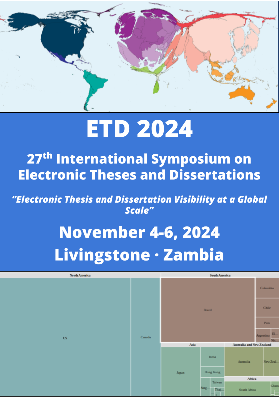
\includepdf{cover}	% our cover was produced with canva.com
	
	
% % % % % % BLANK PAGE
% % % % % %---------------------------------------------------------------------
% % % % % \mbox{}
% % % % % \thispagestyle{empty}
% % % % % \vfill
% % % % % \begin{center}
% % % % % 	\ifOnline
% % % % % 	The electronic version of this booklet can be found at: \\
% % % % % 	https://amcosconference.com/
% % % % % 	\else
% % % % % 	This is the short version of the booklet for print use. Full abstracts with all authors, references, and figures can be found in the electronic version at \url{https://amcosconference.com/}
% % % % % 	\fi % end if
% % % % % 	\\[20pt] % Please cite us by keeping the following line.
% % % % % 	The open-source \LaTeX{} template, AMCOS\_booklet, used to generate this booklet is available at \url{https://github.com/maximelucas/AMCOS\_booklet}
% % % % % \end{center}
% % % % %
% % % % % \newpage

% TABLE OF CONTENTS 
%---------------------------------------------------------------------
\tableofcontents{}

% ABOUT
%---------------------------------------------------------------------
\chapter{About}

\section{27th International Symposium on Eletronic Theses and Dissertations}
The 27th International Symposium on Electronic Theses and Dissertations (ETD 2024) aims to bring together global leaders and researchers working in the broad areas of digital libraries, institutional repositories, scholarly research and electronic theses and dissertations. The theme of ETD 2024 is "ETD Visibility at a Global Scale", and will explore innovative approaches that make use of Electronic Theses and Dissertations (ETDs), including the use of modern-day Artificial Intelligence techniques such as Large Language Models and exploration of advances that will result in increased visibility of ETDs at a Global Scale.

Thank you so very much for coming to Livingstone, Zambia to participate in the ETD 2024 conference events. We sincerely hope you enjoy the conference and your short stay in Livingstone, and, more importantly have productive and worthwhile discussions and meet new people!

Zikomo Kwambili!

\begin{minipage}[t]{\textwidth}
\raggedleft
Best Wishes\\
Lighton Phiri (Chair)
\end{minipage}

\newpage
\section{Local Conference Organizing committee}
\begin{center}
\begin{tabular}{lll}
Lighton Phiri, UNZA & Denny Nsokolo, HEA & Francina Makondo, UNZA \\
Phyela Mbewe, UNZA & Thabiso Mwiinga, UNZA &  Kaoma Daka, UNZA \\
Matildah Muchinga, LAMU  & Stein Mkandawire, ZAMREN & Buumba Dubeka, ZCAS \\
Adrian Chisale, UNZA & Dokowe Tembo, ZCAS & Cecilia Kasonde, KNU \\
Habeenzu Mulunda, UNZA & Francis Kawesha, HEA & Fabian Kakana, UNZA \\
Brian Munkondya, MU & Elijah Chileshe, UNZA & Mpande Ntumbo, ZAMREN \\
\end{tabular}

\section{Volunteers}
\begin{center}
\begin{tabular}{lll}
Mubanga Chibesa, UNZA & Gift Muwele, UNZA & Lwiimwe Shansonga, UNZA \\
Albertina Mooka, UNZA & Christabel Kunda, UNZA &  \\

\end{tabular}

\section{Programme committee}
\begin{center}
\begin{tabular}{lll}
Ana Pavani & Pontifícia Universidade Católica do Rio de Janeiro \\
Charles Greenberg & NDLTD \\
Edward Fox & Virginia Tech \\
Gabriela Mejias & DataCite \\
Hussein Suleman & University of Cape Town \\
Iryna Kuchma & EIFL \\
Jian Wu & Old Dominion University \\
Joachim Schöpfel & University of Lille \\
Lazarus Matizirofa & University of the Witwatersrand \\
Lighton Phiri & University of Zambia \\
Maïté Roux & ABES \\
Mirjana Brkovic & University of Novi Sad \\
Nabi Hasan & Indian Institute of Technology Delhi \\
Ramesh Gaur & Indira Gandhi National Centre for the Arts \\
Shantashree Sengupta & P.E.S Modern College of Arts Science and Commerce \\
Tainá Batista De Assis & Brazilian Institute of Information in Science and Technology \\
William Ingram & Virginia Polytechnic Institute and State University \\
\end{tabular}

\end{center}


% SPONSORS
%------------------------------------------------------------------
\chapter{Partner Institutions and Sponsors}

\begin{center}
The ETD 2024 conference was organised by the Networked Digital Library of Theses and Dissertations (NDLTD) and, additionally hosted by The University of Zambia (UNZA) and co-hosted by The Higher Education Authority (HEA) of Zambia and Zambia Research and Education Network (ZAMREN).
\end{center}

\section{Gold, Silver and Bronze Sponsors}

\begin{center}

\includegraphics[width=0.30\textwidth]{images/logos/Partnerlogos/img-etd24-artwork-sponsors-proquest.png}

\includegraphics[width=0.30\textwidth]{images/logos/Partnerlogos/img-etd24-artwork-sponsors-ebsco.png}

\includegraphics[width=0.40\textwidth]{images/logos/Partnerlogos/img-etd24-artwork-sponsors-datacite.png}

\includegraphics[width=0.30\textwidth]{images/logos/Partnerlogos/img-etd24-artwork-sponsors-uks.png}

\includegraphics[width=0.30\textwidth]{images/logos/Partnerlogos/img-etd24-artwork-sponsors-crossref.jpg}
\includegraphics[width=0.30\textwidth]{images/logos/Partnerlogos/img-etd24-artwork-sponsors-zynle.png}
\end{center}


\section{Partner Institutions/Organisations}

\begin{center}

\includegraphics[width=0.18\textwidth]{images/logos/Partnerlogos/img-etd2024-ndltd_logo.png}

\includegraphics[width=0.10\textwidth]{images/logos/Partnerlogos/img-etd2024-unza_logo.png}

\includegraphics[width=0.18\textwidth]{images/logos/Partnerlogos/img-etd2024-hea_logo.png}

\includegraphics[width=0.25\textwidth]{images/logos/Partnerlogos/img-etd2024-zamren_logo.png}
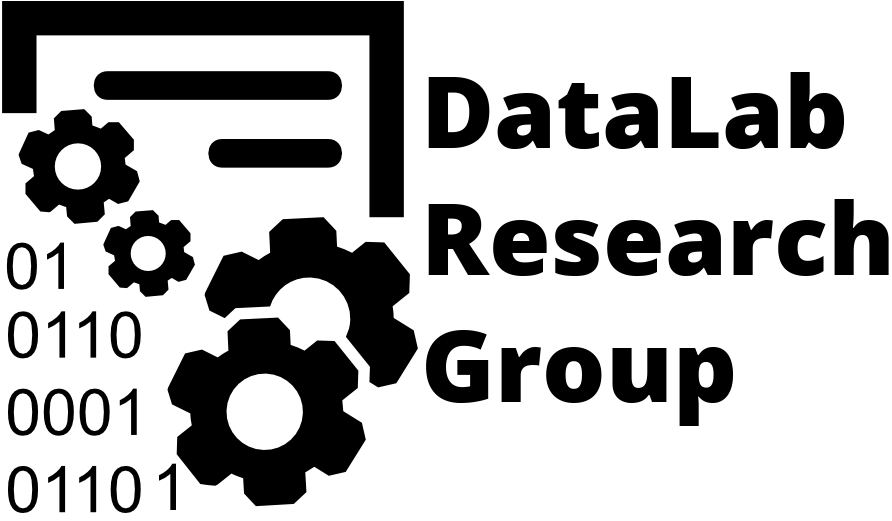
\includegraphics[width=0.18\textwidth]{images/logos/Partnerlogos/img-etd24-artwork-sponsors-datalab.png}
\end{center}


% % % % % % % % % % \vfill
% % % % %
% % % % % \section{Gold Sponsors}
% % % % %
% % % % % \begin{center}
% % % % % 
\includegraphics[width=0.20\textwidth]{images/logos/Partnerlogos/img-etd24-artwork-sponsors-proquest.png}
% % % % % \end{center}
% % % % %
% % % % % \section{Silver Sponsors}
% % % % %
% % % % % \begin{center}
% % % % % 
\includegraphics[width=0.15\textwidth]{images/logos/Partnerlogos/img-etd24-artwork-sponsors-ebsco.png}
% % % % % \end{center}
% % % % %
% % % % % \section{Bronze Sponsors}
% % % % %
% % % % % \begin{center}
% % % % % 
\includegraphics[width=0.15\textwidth]{images/logos/Partnerlogos/img-etd24-artwork-sponsors-datacite.png}
% % % % % 
\includegraphics[width=0.15\textwidth]{images/logos/Partnerlogos/img-etd24-artwork-sponsors-uks.png}
% % % % % 
\includegraphics[width=0.15\textwidth]{images/logos/Partnerlogos/img-etd24-artwork-sponsors-crossref.jpg}
% % % % % \includegraphics[width=0.15\textwidth]{images/logos/Partnerlogos/img-etd24-artwork-sponsors-zynle.png}
% % % % % \end{center}
% % % % %
% % % % % \section{Additional Sponsors}
% % % % %
% % % % % \begin{center}
% % % % % 
\includegraphics[width=0.10\textwidth]{images/logos/Partnerlogos/img-etd2024-ndltd_logo.png}
% % % % % 
\includegraphics[width=0.10\textwidth]{images/logos/Partnerlogos/img-etd2024-unza_logo.png}
% % % % % 
\includegraphics[width=0.10\textwidth]{images/logos/Partnerlogos/img-etd2024-hea_logo.png}
% % % % % 
\includegraphics[width=0.10\textwidth]{images/logos/Partnerlogos/img-etd2024-zamren_logo.png}
% % % % % 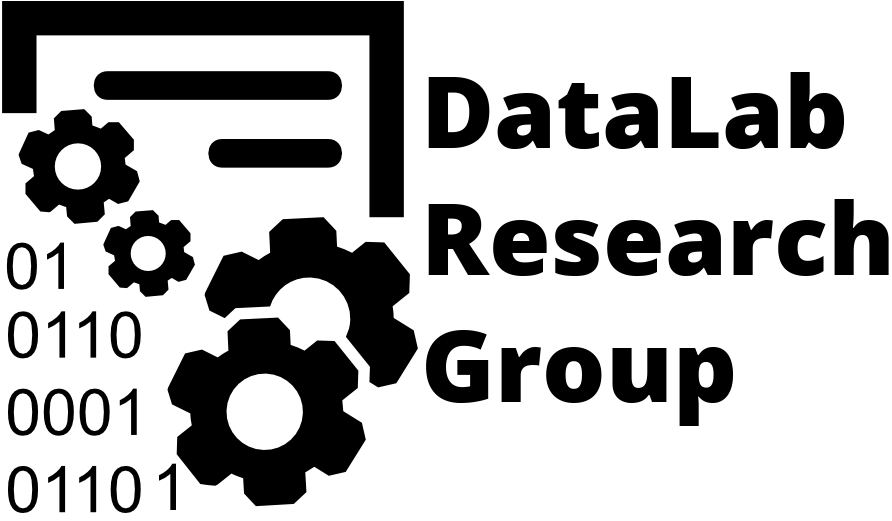
\includegraphics[width=0.10\textwidth]{images/logos/Partnerlogos/img-etd24-artwork-sponsors-datalab.png}
% % % % % \end{center}
% % % % %
% % % % % % % % % % \vfill


\newpage

% TIMETABLE 
%---------------------------------------------------------------------
% \chapter{Timetable}

% CT: Contributed Talk, IS: Invited Speaker, KL: Keynote Lecture, IT: Invited Talk.
% % % Custom commands used here can be found at the end of the preamble_booklet.tex file
% \section{Day 1. Monday, November 4, 2024}

% \begin{center}
% % % % % % 	\filbreak
% \begin{longtable}{|C{0.15\linewidth}| C{0.04\linewidth}|  C{0.3\linewidth} C{0.0\linewidth} C{0.4\linewidth}|}\hline	
% % % % % % 	\tablebreak{}{Day 1. Monday, November 4, 2024}
% 	\tablebreak{8:30--9:00}{Registration}
% 	\CT{08:30--10:00}{Charles Greenberg, Hussein Suleman, Lighton Phiri}{}{NDLTD}{Workshop 1. ETDs 101: No Experience Required!}
% 	\CT{08:30--10:00}{Lombe Tembo}{}{ORCID}{Workshop 2. Leveraging ORCID's Global Participation Program}
% 	\tablebreak{10:00--10:15}{Tea/Coffee}
% 	\IT{10:15--10:25}{Ernest Banda}{}{Zynle Technologies Limited}{Sponsor Talk}
% 	\CT{10:30--13:00}{Charles Greenberg, Hussein Suleman, Lighton Phiri}{}{NDLTD}{Workshop 1. ETDs 101: No Experience Required!}
% 	\CT{10:15--13:00}{Lombe Tembo}{}{ORCID}{Workshop 2. Leveraging ORCID's Global Participation Program}
% 	\tablebreak{13:00--14:00}{Lunch}
% 	\CT{14:00--16:00}{Gabriela Mejias, Olatunbosun Obileye}{}{DataCite}{Workshop 3. DataCite Connect}
% 	\CT{14:00--16:00}{Yinlin Chen, Bill Ingram, Ed Fox}{}{Virginia Tech}{Workshop 4. Globalizing Knowledge}
% 	\tablebreak{16:00--16:15}{Tea/Coffee}
% 	\CT{16:15--18:00}{Gabriela Mejias, Olatunbosun Obileye}{}{DataCite}{Workshop 3. DataCite Connect}
% 	\CT{16:15--18:00}{Yinlin Chen, Bill Ingram, Ed Fox}{}{Virginia Tech}{Workshop 4. Globalizing Knowledge}
% 	\eventtype{18:15--20:00}{NDLTD Board of Directors Meeting}
% 	\eventtype{18:00--20:00}{University of Zambia Ranking Committee Meeting}
% \end{longtable}
% \end{center}


% \section{Day 2. Tuesday, November 5, 2024}

% \begin{center}
% % % % % % 	\filbreak
% \begin{longtable}{|C{0.15\linewidth}| C{0.04\linewidth}|  C{0.3\linewidth} C{0.0\linewidth} C{0.4\linewidth}|}\hline
% % % % % % 	\tablebreak{}{Day 2. Tuesday, November 5, 2024}
% 	\tablebreak{07:30--18:00}{Registration}
% 	\eventtype{08:30--09:45}{Opening Ceremony}
% 	\eventtype{}{Chair: Habeenzu Mulunda}
% 	\eventtype{}{Venue: Convention Centre - Giraffe}
% 	\tablebreak{08:30--08:35}{National Anthem}
% 	\tablebreak{08:35--08:40}{Prayer}
% 	\IS{08:40--08:50}{Lighton Phiri}{}{Chair, ETD 2024}{Welcome Remarks}
% 	\IS{08:50--09:00}{Edward A. Fox}{}{Executive Director, NDLTD}{Opening Remarks}
% 	\IS{09:00--09:10}{Stein Mkandawire}{}{CEO, Zambia Research Education Network}{Remarks}
% 	\IS{09:10--09:20}{Trywell Kalusopa}{}{DVC of Research and Innovation, University of Zambia}{Remarks}
% 	\IS{09:20--09:40}{Kazhila C. Chinsembu}{}{Director General, Higher Education Authority}{Welcome Speech}
% 	\KL{09:40--10:50}{Hussein Suleman}{}{University of Cape Town}{Resilience and ETD Repositories in Poor Countries}

% 	\eventtype{10:50--11:05}{A Moment to Remember: Official Conference Photo}

% 	\tablebreak{11:05--11:20}{Tea/Coffee}

% 	\IT{11:20--11:35}{Sylvia Kgorane}{}{ProQuest, a Part of Clarivate}{Sponsor Talk}
% 	\IT{11:35--11:45}{Deane Kearns}{}{EBSCO Information Services}{Sponsor Talk}
% 	\IT{11:45--11:55}{Sanele Silungile Dlamini}{}{Universal Knowledge Software}{Sponsor Talk}

% 	\eventtype{12:00--13:00}{Session 1A. Infrastructure and Technologies}
% 	\eventtype{}{Chair: Charles Greenberg}
% 	\eventtype{}{Venue: Convention Centre - Giraffe}
% 	\CT{12:00--12:20}{Vivek Ranjan}{}{INFLIBNET}{Landscape of Open Access Repositories with Special Reference to Electronic Theses and Dissertations (ETD) across SAARC and BRICS Nations: A Comparative Analysis}
% 	\CT{12:20--12:40}{Kamani Perera}{}{Chartered Institute of Personnel Management}{Implementing Persistent Identifier Infrastructure for Effective Management of ETD Repositories: A Case Study from Chartered Institute of Personnel Management, Sri Lanka}
% 	\IT{12:40--13:00}{Fitzwell Kabunda}{}{Bridging Gap Solutions}{Invited Talk}

% 	\eventtype{12:00--13:00}{Session 1B. Policies and Practices}
% 	\eventtype{}{Chair: Gabriela Mejias}
% 	\eventtype{}{Venue: Convention Centre - Zebra}
% 	\CT{12:00--12:20}{Shahzeb Hassan}{}{Akal University}{Future-Proofing Research by Long-term ETD Preservation: Challenges and Opportunities}
% 	\CT{12:20--12:40}{Jive Lubbungu}{}{Kwame Nkrumah University}{E-Theses and Dissertations in Zambia: A Case Study of Two Universities in Kabwe}
% 	\CT{12:40--13:00}{Kamani Perera}{}{Chartered Institute of Personnel Management}{Nurturing Advanced Research Culture among Medical Practitioners through ETDs: A case study from University of Kelaniya, Sri Lanka}

% 	\tablebreak{13:00--14:00}{Lunch}

% 	\eventtype{14:00--15:30}{Session 2A. Impact and Utilisation}
% 	\eventtype{}{Chair: Olatunbosun Obileye}
% 	\eventtype{}{Venue: Convention Centre - Zebra}
% 	\CT{14:00--14:20}{Brenda Van Wyk}{}{University Of Pretoria}{Do More Complete Dissertations' Metadata Get More Engagement?}
% 	\CT{14:20--14:40}{Mark E Phillips}{}{University Of North Texas}{Extracting and Registering References to Improve Scholarly Impact of ETDs}
% 	\CT{14:40--15:00}{Ana M B Pavani}{}{Pontifícia Universidade Católica do Rio de Janeiro}{International Visibility of ETDs in Portuguese and in English on a Brazilian Repository}
% 	\CT{15:00--15:20}{Zillur Rahman}{}{Ahsanullah University of Science and Technology}{Designing a plan for sharing ETD among the University Libraries in Bangladesh}

% 	\eventtype{14:00--15:30}{Session 2B. ETDs in Developing Countries}
% 	\eventtype{}{Chair: Hussein Suleman}
% 	\eventtype{}{Venue: Convention Centre - Giraffe}
% 	\CT{14:00--14:20}{Joseph P Telemala}{}{Sokoine University Of Agriculture}{Improving the Mkulima Repository Content: Utilizing Theses, Dissertations, and LLMs for Agricultural Knowledge Dissemination in Kiswahili}
% 	\CT{14:20--14:40}{Kenneth K Rotich}{}{Egerton University}{The Changing Landscape in Research Data Management in Kenya’s Universities: An Analysis of Development and Implementation}
% 	\CT{14:40--15:00}{Kamani Perera}{}{Chartered Institute Of Personnel Management}{Empowering HRM Professionals: Advancing Research Culture with ETDs in The Chartered Institute of Personnel Management (CIPM), Sri Lanka}
% 	\CT{15:00--15:20}{Kamani Perera}{}{Chartered Institute Of Personnel Management}{Unlocking the Potential of ETDs: Implementation Novel ETD Repository in Chartered Institute of Personnel Management in Sri Lanka}

% 	\tablebreak{15:30--15:45}{Tea/Coffee}

% 	\eventtype{15:45--17:00}{Session 3A. Infrastructure and Technologies}
% 	\eventtype{}{Chair: Kaoma Daka}
% 	\eventtype{}{Venue: Convention Centre - Giraffe}
% 	\CT{15:45--16:05}{Elijah Chileshe}{}{University of Zambia}{A Pre-Processing Pipeline for Improved ETD Metadata Quality in Downstream Services}
% 	\CT{16:05--16:25}{Adrian Chisale}{}{University of Zambia}{Seamless Integration of Koha and DSpace for Enhanced Management of Theses and Dissertations in Hybrid Environment: a case of University of Zambia Library}

% 	\eventtype{15:45--17:00}{Session 3B. ETDs in Developing Countries}
% 	\eventtype{}{Chair: Fabian Kakana}
% 	\eventtype{}{Venue: Convention Centre - Zebra}
% 	\CT{15:45--16:05}{Mpundu Chilonga}{}{Kwame Nkruma University}{Examining the Cultural and Institutional Factors Impacting ETD Visibility in Zambia: Policy and Practice Implications}
% 	\CT{16:05--16:25}{Lamia Salsabil}{}{Old Dominion University}{ETD MS v2.0: A New Schema Draft for Electronic Theses and Dissertations}

% 	\eventtype{19:00--22:00}{Mukuni BOMA Cultural Experience Welcome Reception}
% 	\eventtype{}{Chair: Habeenzu Mulunda}
% 	\eventtype{}{Venue: Mukuni BOMA}
% \end{longtable}
% \end{center}



% \section{Day 3. Wednesday, November 6, 2024}

% \begin{center}
% % % % % % 	\filbreak
% \begin{longtable}{|C{0.15\linewidth}| C{0.04\linewidth}|  C{0.3\linewidth} C{0.0\linewidth} C{0.4\linewidth}|}\hline
% % % % % % 	\tablebreak{}{Day 3. Wednesday, November 6, 2024}
% 	\tablebreak{07:30--18:00}{Registration}

% 	\eventtype{08:30--09:30}{Session 4A. Invited Talks: ETD Initiatives in Zambia}
% 	\eventtype{}{Chair: Denny Nsokolo}
% 	\eventtype{}{Venue: Convention Centre - Giraffe}
% 	\IS{08:30--08:40}{Mosebjadi Petje}{}{Times Higher Education}{University Ranking}
% 	\IT{08:45--08:55}{Johanssen Obanda}{}{Crossref}{Sponsor Talk}
% 	\IS{09:00--09:10}{Benaia Akombwa}{}{University of Zambia}{Scholarly Research Infrastructure}
% 	\IS{09:15--09:25}{Zachary Zulu}{}{University of Zambia}{University of Zambia Institutional Repository}
% 	\IS{09:30--09:40}{Clement Sinyangwe}{}{Chalimbana University}{Chalimbana University Institutional Repository}
% 	\IS{09:45--09:55}{Buumba Dubeka and Dokowe Tembo}{}{ZCAS University}{ZCAS University Institutional Repository}
% 	\IS{10:00--10:10}{Mpundu Chilonga and Cecilia Kasonde}{}{Kwame Nkruma University}{Kwame Nkruma University Institutional Repository}

% 	\eventtype{10:10--11:30}{Session 5A. Panel Discussion}
% 	\eventtype{}{Chair: Dokowe Tembo}
% 	\eventtype{}{Venue: Convention Centre - Giraffe}
% 	\IT{10:10--11:30}{How do we set up Successful ETD Projects in Zambia?}{}{Moderator: Hussein Suleman}{Participants: \hspace{5cm} Gabriela\,Mejias (DataCite) $\cdot$ Manoj\,Kumar (INFLIBNET) $\cdot$ Lighton\,Phiri (UNZA) $\cdot$ Zachary\,Zulu (UNZA)}

% 	\eventtype{11:30--12:00}{Session 6A. Poster/Demo Session: Minute Madness}
% 	\eventtype{}{Chair: Lombe Tembo}
% 	\eventtype{}{Venue: Convention Centre - Giraffe}
% 	\CT{11:30--11:32}{Kamani Perera}{}{Chartered Institute of Personnel Management}{Enhancing Access to Scholarly Knowledge: Strategies for Promoting Open Access ETDs in Sri Lanka}
% % % % % % 	\CT{11:02--11:04}{Okhakhu O. David}{}{Lead City University}{Enhancing Electronic Thesis and Dissertation Visibility: A Focus on Institutional Repository Platforms and Inherent Challenges in the Nigerian Context}
% 	\CT{11:32--11:34}{Kamani Perera}{}{Chartered Institute of Personnel Management}{Total Quality Management in ETD Repository at Chartered Institute of Personnel Management (CIPM)}
% 	\CT{11:35--11:37}{Martin C Musonda}{}{University of Zambia}{Automatic Summarisation of Electronic Theses and Dissertations for Increased Media Engagement}
% 	\CT{11:38--11:40}{Lwiime Shansonga}{}{University of Zambia}{Automatic Electronic Thesis and Dissertation Guideline Verification For Consistently Formatted Manuscripts}
% 	\CT{11:41--11:43}{Elijah Chileshe}{}{University of Zambia}{Design and Implementation of an Interoperable Zambia National Electronic Thesis and Dissertation Portal}
% 	\CT{11:44--11:46}{Vivek Mr Ranjan}{}{INFLIBNET Center}{Exploring AI-driven strategies for enhancing the visibility of E-Theses in Shodhganga Repository}
% % % % % % 	\CT{11:14--11:16}{Rajabu Mr Simba}{}{AHILA}{Assessing the Efficiency of Data Science Programs in Enhancing Big Data Analysis Skills among Health Libraries and Information Scientists}
% % % % % % 	\CT{11:16--11:18}{Zainabu H LILUTU}{}{Mbeya University of Science and Technology}{Optimizing Electronic Theses and Dissertations Management for Broad Audience Engagement at Dr. Magufuli Library of Mbeya University of Science and Technology, Tanzania}
% 	\CT{11:47--11:49}{Zillur Rahman}{}{Ahsanullah University of Science and Technology}{Determining the factors influencing the utilization of open source digital repository software in the preservation of ETDs in academic libraries in Bangladesh}
% 	\CT{11:50--11:52}{Zillur Rahman}{}{Ahsanullah University of Science and Technology}{ETDs in Ensuring Quality Education for Economic Growth to Achieve Sustainable Development Goals (SDGs): Experience of SAARC Countries}
% 	\CT{11:53--11:55}{Mutali M Lithole}{}{University Of Johannesburg}{The University of Johannesburg’s journey to enhance the content of the Institutional Repository (IR) and improve discoverability}
% 	\CT{11:56--11:58}{Mduduzi Ntetha}{}{UNISA}{The conversion of printed theses and dissertations into digital formats: A case study of the University of South Africa library}
% % % % % % 	\CT{11:26--11:28}{Sukanta  Kumar Patra}{}{Vidyasagar College for Women}{Global Visibility of National ETD Repositories of G20 Countries: comparative studies with respect to NDLTD's meta repository}
% % % % % % 	\CT{11:28--11:30}{M A M Mominur Rahman}{}{University Of Rajshahi}{Managing ETDs in Rajshahi University Central Library : Problems and Possibilities}
% 	\CT{11:59--12:00}{Nobbie kandira}{}{Zimbabwe Open University}{Creating an ETD database using OMEKA. The Zimbabwe Open University Experience}

% 	\tablebreak{12:00--12:30}{Tea/Coffee}
% 	\eventtype{12:00--12:30}{Session 7A. Poster Session with Tea/Coffee}
% 	\eventtype{}{Chair: Thabiso Mwiinga}
% 	\eventtype{}{Venue: Convention Centre}

% 	\eventtype{12:30--13:00}{Closing Ceremony}
% 	\eventtype{}{Chair: Buumba Dubeka}
% 	\eventtype{}{Venue: Convention Centre - Giraffe}
% 	\IT{12:30--12:45}{Charles Greenberg}{}{Representative - NDLTD}{NDLTD Updates}
% 	\IT{12:45--13:00}{John Hagen}{}{Executive Director - USETDA}{ETD 2025 Presentation}
% 	\IT{12:30--12:45}{Lighton Phiri}{}{Chair - ETD 2024}{Closing Remarks}

% 	\tablebreak{13:00--14:00}{Lunch}

% 	\eventtype{14:00--15:00}{Mukuni Village Tour}
% 	\eventtype{14:00--15:00}{Victoria Falls Tour}
% \end{longtable}
% \end{center}


% TALKS 
%---------------------------------------------------------------------
% \chapter{List of Abstracts}
\chapter{Full Papers Track}

\input{abstracts/tex/f\type_53_telemala}
\input{abstracts/tex/f\type_43_lubbungu}
\input{abstracts/tex/f\type_29_rahman}
\input{abstracts/tex/f\type_7_perera}
\input{abstracts/tex/f\type_15_perera}
\input{abstracts/tex/f\type_16_pavani}
\input{abstracts/tex/f\type_45_salsabil}
\input{abstracts/tex/f\type_18_ranaweera}
\input{abstracts/tex/f\type_56_hasan}
\input{abstracts/tex/f\type_23_wyk}
\input{abstracts/tex/f\type_38_sousa}
\input{abstracts/tex/f\type_44_phillips}
\input{abstracts/tex/f\type_22_chilonga}
\input{abstracts/tex/f\type_4_rotich}
\input{abstracts/tex/f\type_6_perera}
\input{abstracts/tex/f\type_40_ranjan}
\input{abstracts/tex/f\type_48_chileshe}
\input{abstracts/tex/f\type_28_rahman}

\chapter{Posters Track}

\input{abstracts/tex/p\type_55_kandira}
\input{abstracts/tex/p\type_51_saikia}
\input{abstracts/tex/p\type_47_chileshe}
\input{abstracts/tex/p\type_46_shansonga}
\input{abstracts/tex/p\type_33_musonda}
\input{abstracts/tex/p\type_27_perera}
\input{abstracts/tex/p\type_11_okhakhu}
\input{abstracts/tex/p\type_8_perera}
\input{abstracts/tex/p\type_2_simba}
\input{abstracts/tex/p\type_9_lithole}
\input{abstracts/tex/p\type_12_ntetha}
\input{abstracts/tex/p\type_13_patra}
\input{abstracts/tex/p\type_14_rahman}

% \section{Workshops}

% Definitions of custom environment used here can be found in preamble_booklet.tex file

% The following input commands automatically select the right version
% (print or online) version of the abstract's .tex
% \type is defined in preamble_booklet.tex and equals:
% 'o' (online) or 'p' (print)

% \input{abstracts/tex/w\type_34_greenberg}
% \input{abstracts/tex/w\type_26_mejias}
% \input{abstracts/tex/w\type_24_chen}
% \input{abstracts/tex/w\type_17_tembo}

% \section{Full Papers}

% Definitions of custom environment used here can be found in preamble_booklet.tex file

% The following input commands automatically select the right version 
% (print or online) version of the abstract's .tex
% \type is defined in preamble_booklet.tex and equals:
% 'o' (online) or 'p' (print)



% POSTERS
%------------------------------------------------------------------
% % % % % \chapter{List of Posters}

% \vspace{-2.5em}
% \newpage
% \section{Posters}



% \section{Invited Talks}

% \input{abstracts/tex/i\type_00_suleman}
% \input{abstracts/tex/i\type_00_petje}

% LIST OF PARTICIPANTS
%------------------------------------------------------------------
\chapter{Authors Index}
 
% The array below was automatically created from a spreadsheet with 'calc2latex'

\begin{center}
\rowcolors{1}{gray!25}{white}
\begin{longtable}{p{0.28\linewidth} p{0.4\linewidth} p{0.25\linewidth}}
\toprule
\textbf{Delegate Name} & \textbf{Organisation} & \textbf{Country} \\
\usepackage{booktabs}
\midrule
Andy Neale & Clarivate & United Kingdom \\  \hline
Austin Mclean & ProQuest, a part of Clarivate & United States \\  \hline
Benaiah Akombwa & University of Zambia & Zambia \\  \hline
Bertrand Thomas & Abes & France \\  \hline
Birbal Boniface Musoba & Higher Education Authority & Zambia \\  \hline
Boniface Banda & The University of Zambia & Zambia \\  \hline
Brenda Van Wyk & University of Pretoria & South Africa \\  \hline
Cecilia Kasonde & Kwame Nkrumah University & Zambia \\  \hline
Charles Greenberg & Networked Digital Library of Theses and Dissertations & United States \\  \hline
Denny Nsokolo & Higher Education Authority & Zambia \\  \hline
Dokowe Tembo & ZCAS University & Zambia \\  \hline
Douglas Mwale & St Bonaventure University & Zambia \\  \hline
Dr Beatrice May Banda & Chipata College of Nursing and Midwifery & Zambia \\  \hline
Edward Fox & Networked Digital Library of Theses and Dissertations (NDLTD) & United States \\  \hline
Efraim Dumeni & Namibia University of Science and Technology & Namibia \\  \hline
Elijah Chileshe & The University of Zambia & Zambia \\  \hline
Elizabeth Namonje & Higher Education Authority & Zambia \\  \hline
Ernest Banda & Zynle Technologies Limited & Zambia \\  \hline
Fabian Kakana & University of Zambia & Zambia \\  \hline
Fitzwell Kabunda & Bridging Gap Solution Limited & Zambia \\  \hline
Francina Makondo & University of Zambia Library & Zambia \\  \hline
Francis Kawesha & Higher Education Authority & Zambia \\  \hline
Gabriela Mejias & DataCite & Germany \\  \hline
Gift Muwele & The University of Zambia & Zambia \\  \hline
Godfrey Marera & St. Bonaventure University & Zambia \\  \hline
Hope Chinganya & CIDRZ & Zambia \\  \hline
Hussein Suleman & University of Cape Town & South Africa \\  \hline
Johanssen Obanda & Crossref & Kenya \\  \hline
Joseph Muyunda Walusiku & Centre for Infectious Disease Research in Zambia & Zambia \\  \hline
Joseph Telemala & Sokoine University of Agriculture & Tanzania \\  \hline
Josiline Chigwada & University of South Africa & South Africa \\  \hline
Kabuku Mwandamena & Chipata College of Nursing and Midwifery & Zambia \\  \hline
Kabwe Kasoma & CIDRZ & Zambia \\  \hline
Kamani Perera & Chartered Institute of Personnel Management & Sri Lanka \\  \hline
Kaoma Lamba Daka & University of Zambia & Zambia \\  \hline
Kazhila C. Chinsembu & Higher Education Authority & Zambia \\  \hline
Kelvin Chibomba (Phd) & Information and Communications zuniversity & Zambia \\  \hline
Kudakwashe Siziva & Datacite & South Africa \\  \hline
Lamia Salsabil & Old Dominion University & United States \\  \hline
Lazarus Matizirofa Banda & University of the Witwatersrand, Johannesburg & South Africa \\  \hline
Lewis Cheelo & Zambia Air Force (ZAF) & Zambia \\  \hline
Lighton Phiri & University of Zambia & Zambia \\  \hline
Lombe Tembo & ORCID & Zambia \\  \hline
Manoj Kumar K & INFLIBNET Centre & India \\  \hline
Mark Phillips & University of North Texas & United States \\  \hline
Martin Mushumba & Higher Education Authority & Zambia \\  \hline
Martin Nkumbula & Zynle Technologies Limited & Zambia \\  \hline
Marvin Kabubi & Information and Communications University & Zambia \\  \hline
Matamela Michael Mulaudzi & University of the Witwatersrand, Johannesburg & South Africa \\  \hline
Matildah Mercy Muchinga & Lusaka Apex Medical University & Zambia \\  \hline
Mduduzi Aubrey Ntetha & University of South Africa & South Africa \\  \hline
Melusi Ncube & Bridging Gap Solutions & Zambia \\  \hline
Mercy Banda & St. Bonaventure University & Zambia \\  \hline
Mosebjadi (Mose) Petje & Times Higher Education & South Africa \\  \hline
Moses Makungu & Zambia Air Force Center of Advance Learning & Zambia \\  \hline
Moses Mupeta & Information and communications university & Zambia \\  \hline
Mpundu Chilonga & KWAME NKRUMAH UNIVERSITY & Zambia \\  \hline
Mubanga Chibesa & The University Of Zambia & Zambia \\  \hline
Olatunbosun Obileye & DataCite & Nigeria \\  \hline
Olivier Cian & ABES & France \\  \hline
Phyela Mbewe & University of Zambia & Zambia \\  \hline
Shahzeb Hasan & Akal University & India \\  \hline
Thabiso Mwiinga-Mwanachingwala & University of Zambia & Zambia \\  \hline
Vivek Ranjan & Silver Oak University & India \\  \hline
Wendel Fabian Chinsamy & DataCite & South Africa \\  \hline
Yinlin Chen & Virginia Tech & United States \\  \hline
Zachary Zulu & THE UNIVERSITY OF ZAMBIA & Zambia \\  \hline
\end{longtable}
\end{center}



% CONFERENCE PROCEEDINGS
%------------------------------------------------------------------
% \chapter{Conference Proceedings}
 
% \section{Posters}
\begin{abstract_online}{Automatic Electronic Thesis and Dissertation Guideline Verification For Consistently Formatted Manuscripts}{%
    \underline{Mubanga C. Chibesa}$^{1}$, Albertina Mooka$^{1}$, Gift Muwele$^{1}$, Lwiime Shansonga$^{1}$, Lighton Phiri$^{1}$}{%
    }{%
    $^1$ The University Of Zambia}

Abstract:

Higher Education Institutions worldwide enforce guidelines and academic approaches to ensure scholarly integrity and adherence to academic standards(Razı et al., 2019).The University of Zambia, is not an exception. Just like most HEIs it offers  training to postgraduate students and one of the key aspects of postgraduate training is producing an Electronic Thesis and Dissertation manuscript The Directorate of Research and Graduate Studies (DRGS) provides guidelines which stipulate how ETD’s should be formatted. Successful graduation is dependent on postgraduate students’ manuscripts of which their conformance to the guidelines is a key aspect. Examiners and other relevant authorities are expected to verify and check if postgraduate students' manuscripts conform to the guidelines.
However, the process of  checking for conformance is a manual and tedious procedure, resulting in submission of inconsistently formatted manuscripts. Although this research seeks to ascertain the exact reasons why this is so, it is apparent that the primary task for the examiners is approving the content written in these manuscripts, and the secondary task being making sure that each and every manuscript is in conformance to the postgraduate guidelines and this is arguably an intense exercise. To address this challenge our  project seeks to implement a tool that will automate the process of checking ETD’s compliance against established postgraduate guidelines. The tool will leverage data mining techniques to perform these tasks. More specifically, document layout analysis (DLA)(Binmakhashen \& Mahmoud, 2019). The tool will flag off portions of ETD manuscripts that do not  conform to established guidelines. Hence, this will help resolve the inconsistencies in the format of submitted manuscripts. 

Methodology:

We will employ a mixed method approach  combining both qualitative and quantitative methods for data collection and analysis. Primary data is being collected through structured interviews and questionnaires, while secondary data involves  document analysis of postgraduate guidelines and archived historical ETDs. Convenient  sampling and purposive sampling  will be used to select participants, the selection is based on judgement and their willingness to participate in the study. The study is targeted on postgraduate examiners, alumni and current postgraduate students. Document analysis will be employed to understand the postgraduate guidelines stipulated in the (The University of Zambia, 2015) document and the identified guidelines are to be categorised into themes and a checklist will be prepared which will be used as a measurement instrument and each guideline, will be set as a question  and each question will be given a measurement scale of 1-5; content analysis will be used on randomly sampled ETDs in order to experimentally determine the extent of the problem using Park’s metrics of metadata quality (accuracy, consistency and completeness) and, finally, a DLA Natural Language Processing model will be implemented and will be evaluated using standard DLA metrics such as Structure Similarity Index and Intersection over Union.
This DLA pipeline is  hinged on Artificial intelligence and Natural language processing(NLP)(Mishra \& Kumar, 2020). We also  leveraged  an open source package called Deepdoctetion for the implementation of the software tool. 
For the development process, Agile methodologies, specifically scrum, will be used for software development, with document layout techniques applied to enhance the Deepdoctetion package in the process. We also accessed the accuracy and usability of the tool through a benchmark dataset composed of historical ETDs archived on The University of Zambia institutional repository. Measurement instruments include structured interview guides and a checklist to evaluate the threshold of compliance of historical ETDs.
Preliminary Findings  and Discussion
Empirical Analysis of Historical Archived ETDs
The analysis of historical archived manuscripts against postgraduate guidelines revealed that most manuscripts did not adhere to the guidelines. The preliminary findings indicate that the majority of the students from all the schools at the institution performed poorly on sections such as the copyright declaration page which had the lowest compliance, with much lower scores in accuracy (2.227), consistency (2.194), and completeness (2.037). This suggests that this section of the manuscripts frequently falls short of meeting the required standards, highlighting a critical area for improvement. This is followed by the declaration page with the second lowest scores in accuracy (3.042), consistency (2.681) and completeness (2.835). The compliance to miscellaneous requirements also had some low scores in accuracy (3.774), consistency (3.760) and completeness (3.841).
Overall middle-ranking sections include the title Page with the following compliance scores in accuracy (4.078), consistency (3.861) and completeness (4.023).  Whereas compliance on the certificate of approval indicates the following scores in accuracy (4.293),consistency (4.304) and completeness (4.322). Similarly, the end matter section with the following compliance scores in accuracy (4.581), consistency (4.471) and completeness (4.551).Lastly, compliance to pagination had the following scores in accuracy (4.634), consistency (4.629) and completeness (4.623). 
However, while these sections generally show good compliance, the moderate degree of variation suggests that there are some inconsistencies in adherence to the guidelines, and targeted improvements could enhance their overall performance.
Overall, the "Order Of Text" demonstrates exceptional compliance with nearly perfect scores in accuracy (4.969), consistency (5) and completeness (5). Similarly, compliance to the prescribed length of an ETD indicates remarkable scores in accuracy (5), consistency (5) and completeness (5).
Survey responses for current postgraduate students
According to the responses from current postgraduate students, the most common challenges in ensuring correct document formatting in accordance with the universities guidelines included difficulties with citation management, generating the correct table of contents, and formatting tables and figures. Out of 22 respondents, seven (7) highlighted that they find difficulties in adjusting their manuscripts to  the prescribed margins, another seven (7) highlighted difficulties when working on tables and figures. Ten respondents stated that the most challenging aspect is with regards to generating references and citations. Five respondents also highlighted that following the prescribed table of contents is challenging for them.
Of the 22 respondents, 50\% stated that they were not very familiar with the postgraduate guidelines of the institution while 6 % stated that they were somewhat familiar with the guidelines. Of the remaining 8%, 4% stated that they were very familiar with the guidelines while the other 4% stated that they were not familiar with the guidelines at all.

Survey results indicate that postgraduate alumni faced challenges with formatting their manuscripts, particularly in adding tables, maps, figures (5 respondents), managing citations (4 respondents), and inserting footnotes (2 respondents). These difficulties align with the low scoring of miscellaneous guidelines (covering citations, figures, and tables) in historical ETD analyses.

Examiners also reported challenges in manually verifying manuscript compliance. With a high student-to-examiner ratio in some schools, the workload can be overwhelming, limiting their ability to be thorough. Due to time constraints, examiners often review up to 50 manuscripts per sitting to provide timely feedback and avoid delaying student research. Furthermore, examiners stated that they find themselves either resending the guidelines to the students or scheduling short seminars mid-research to re-educate the students about the guidelines when they notice a lot of inconsistencies in the  submitted manuscripts.
Conclusion
The use of DLA methods to create a pipeline that will curtail the challenge of ensuring and checking compliance of ETDs to postgraduate guidelines at the university of Zambia has proven to be the most efficient solution. The development of an ETD automatic guideline verification tool presents an opportunity to enhance efficiency as well as promote consistency in the quality of ETDs while alleviating the challenges faced in the process of manually checking for compliance consequently reducing the workload for students, supervisors and examiners alike. 

References:

Mishra, B. K., \& Kumar, R. (2020). Natural Language Processing in Artificial Intelligence.
Razı, S., Glendinning, I., \& Foltýnek, T. (2019). Towards Consistency and Transparency in Academic Integrity. Peter Lang Gmbh, Internationaler Verlag Der Wissenschaften.
Binmakhashen, G. M., \& Mahmoud, S. A. (2019). Document Layout Analysis: A Comprehensive Survey. ACM Comput. Surv., 52(6), 1–36.
The University of Zambia. (2015). Directorate of Research and Graduate Studies: Postgraduate regulations.

\begin{center}
    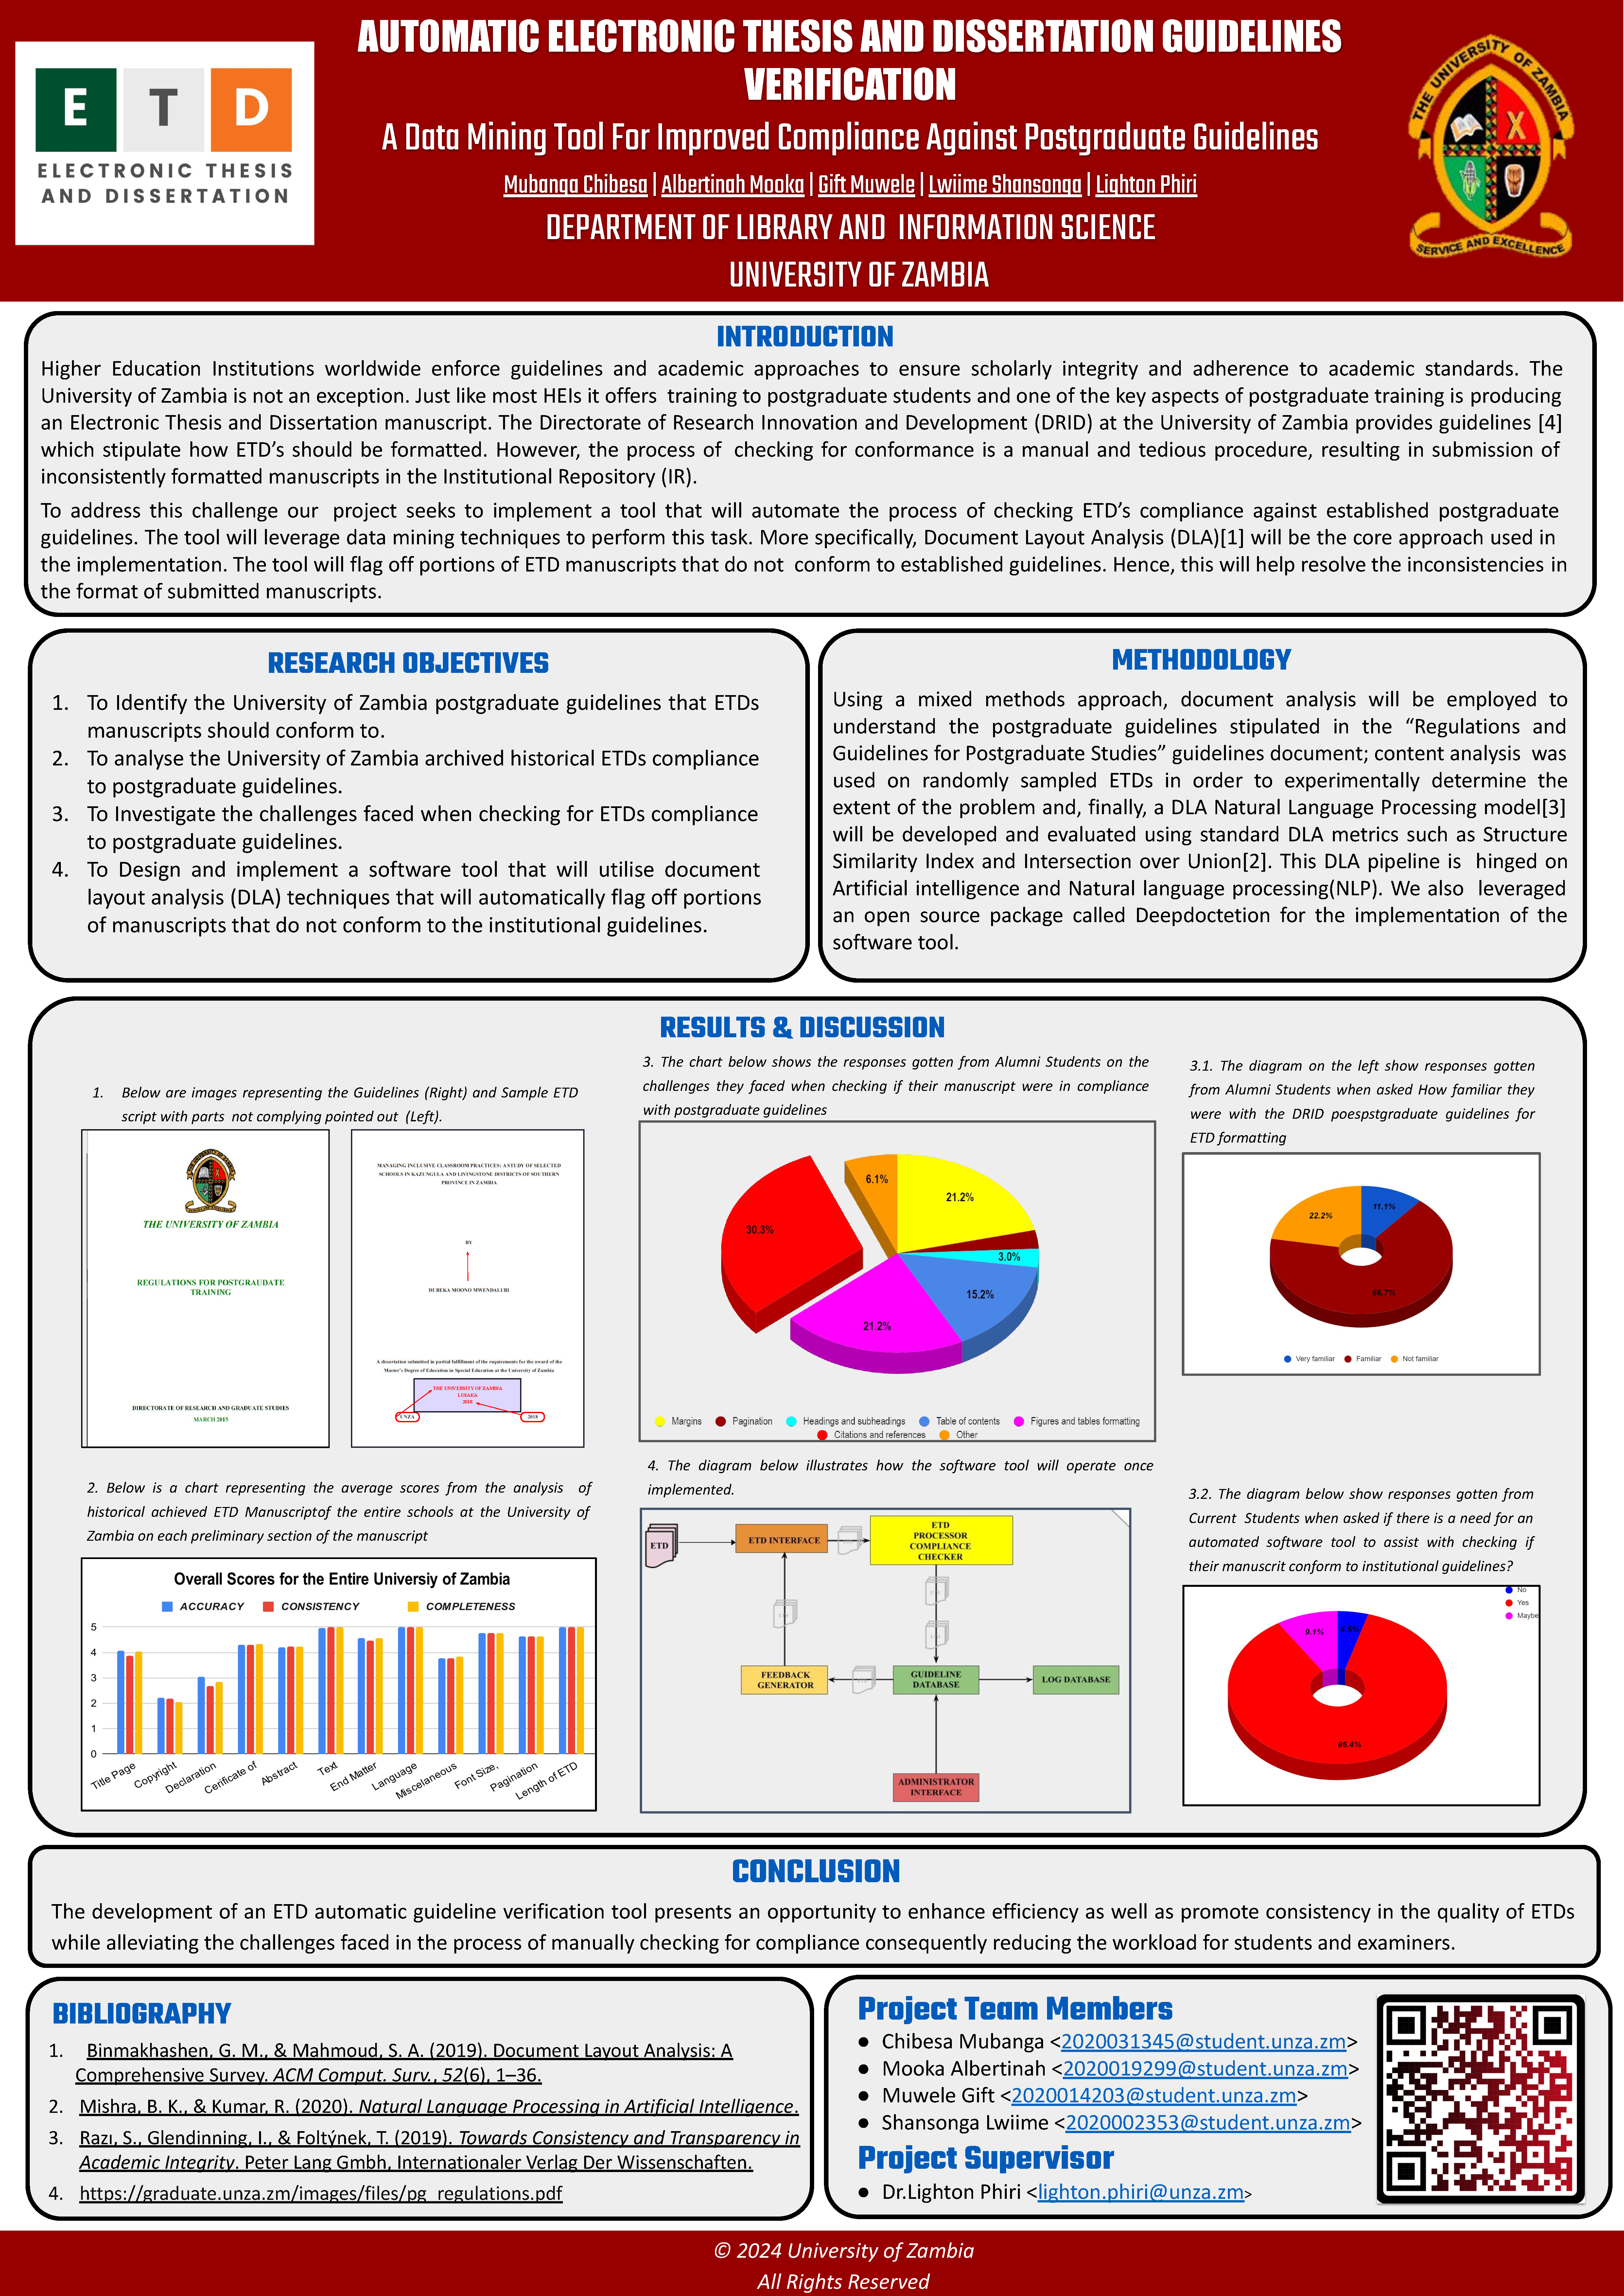
\includepdf[pages=1, width=\linewidth]{./conference_assets/docs-poster-etd24-46}
\end{center}

\end{abstract_online}

%  
% USEFUL INFO
%------------------------------------------------------------------
% \chapter{Useful Information}

% The ETD 2024 conference activities will be held at Avani Victoria Falls' \textbf{Convention Centre}. We shall be using the Zebra and Giraffe conference rooms.

\textbf{Tea/Coffee breaks and lunches} will be offered during the conference.

The \textbf{poster session} will be held on Wednesday, November 6 2024 and will comprise of a \textbf{"one minute madness"}, followed by a textbf{Poster Session with Tea/Coffee}.

Wi-Fi will be available during the conference. The Zambia Research and Education Network will also provide access to an eduroam network throughout the duration of the conference.

The \textbf{conference welcome reception} will be held at the \textbf{Mukuni BOMA Village}, on the banks of the Zambezi River.

\section{How to get to the Avani Victoria Falls Resort?}

Avani Victoria Falls Resort is located on the banks of the Zambezi river with a 5-minute walk direct access to Victoria Falls.

\begin{itemize}

	\item \textbf{Air:} From Lusaka, Kenneth Kaunda International Airport, you can fly directly to Livingstone, Harry Mwaanga Nkumbula International Airport (formerly known as Livingstone Airport). Flights are available with Proflight Zambia (daily flights) or Zambia Airways (daily flights). The journey takes around 1 hour and 10 minutes. Harry Mwaanga Nkumbula International Airport in Livingstone also has direct flights from Johannesburg (JNB), Cape Town (CPT) and Nairobi (NBO), (South Africa and Kenya). Note that the most frequent flights to Livingstone are routes from Lusaka (LUN), domestic, and Johannesburg (JNB), South Africa, with an average of 6 flights per day.
	\item \textbf{Bus:} Various long-distance buses operate daily between Lusaka and Livingstone. Buses leave Lusaka from 6:00 am and every half hour thereafter until 11.30 am. The journey takes around 6 to 7 hours.
	\item \textbf{Getting Around:}
	\begin{itemize}
	    \item \textbf{Taxis}: Taxis are readily available and can be hired for specific trips, for a half-day or for a full-day.
        \item \textbf{Local mini-buses}: There is a network of local mini buses that connect various parts of Livingstone.
    \end{itemize}
	
\end{itemize}

\subsection{Avani Victoria Falls Resort: Google Maps Location}

\begin{center}
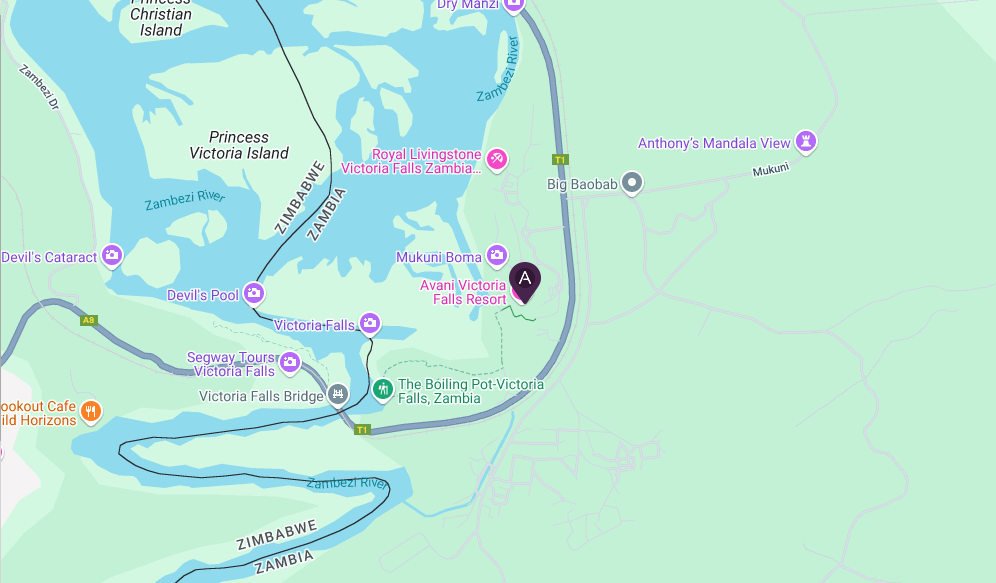
\includegraphics[width=\linewidth]{images/img-etd24-avani_victoria_fall_convention_centre_map.png}
\end{center}


\subsection{Avani Victoria Falls Resort: Convention Centre Layout}

\begin{center}
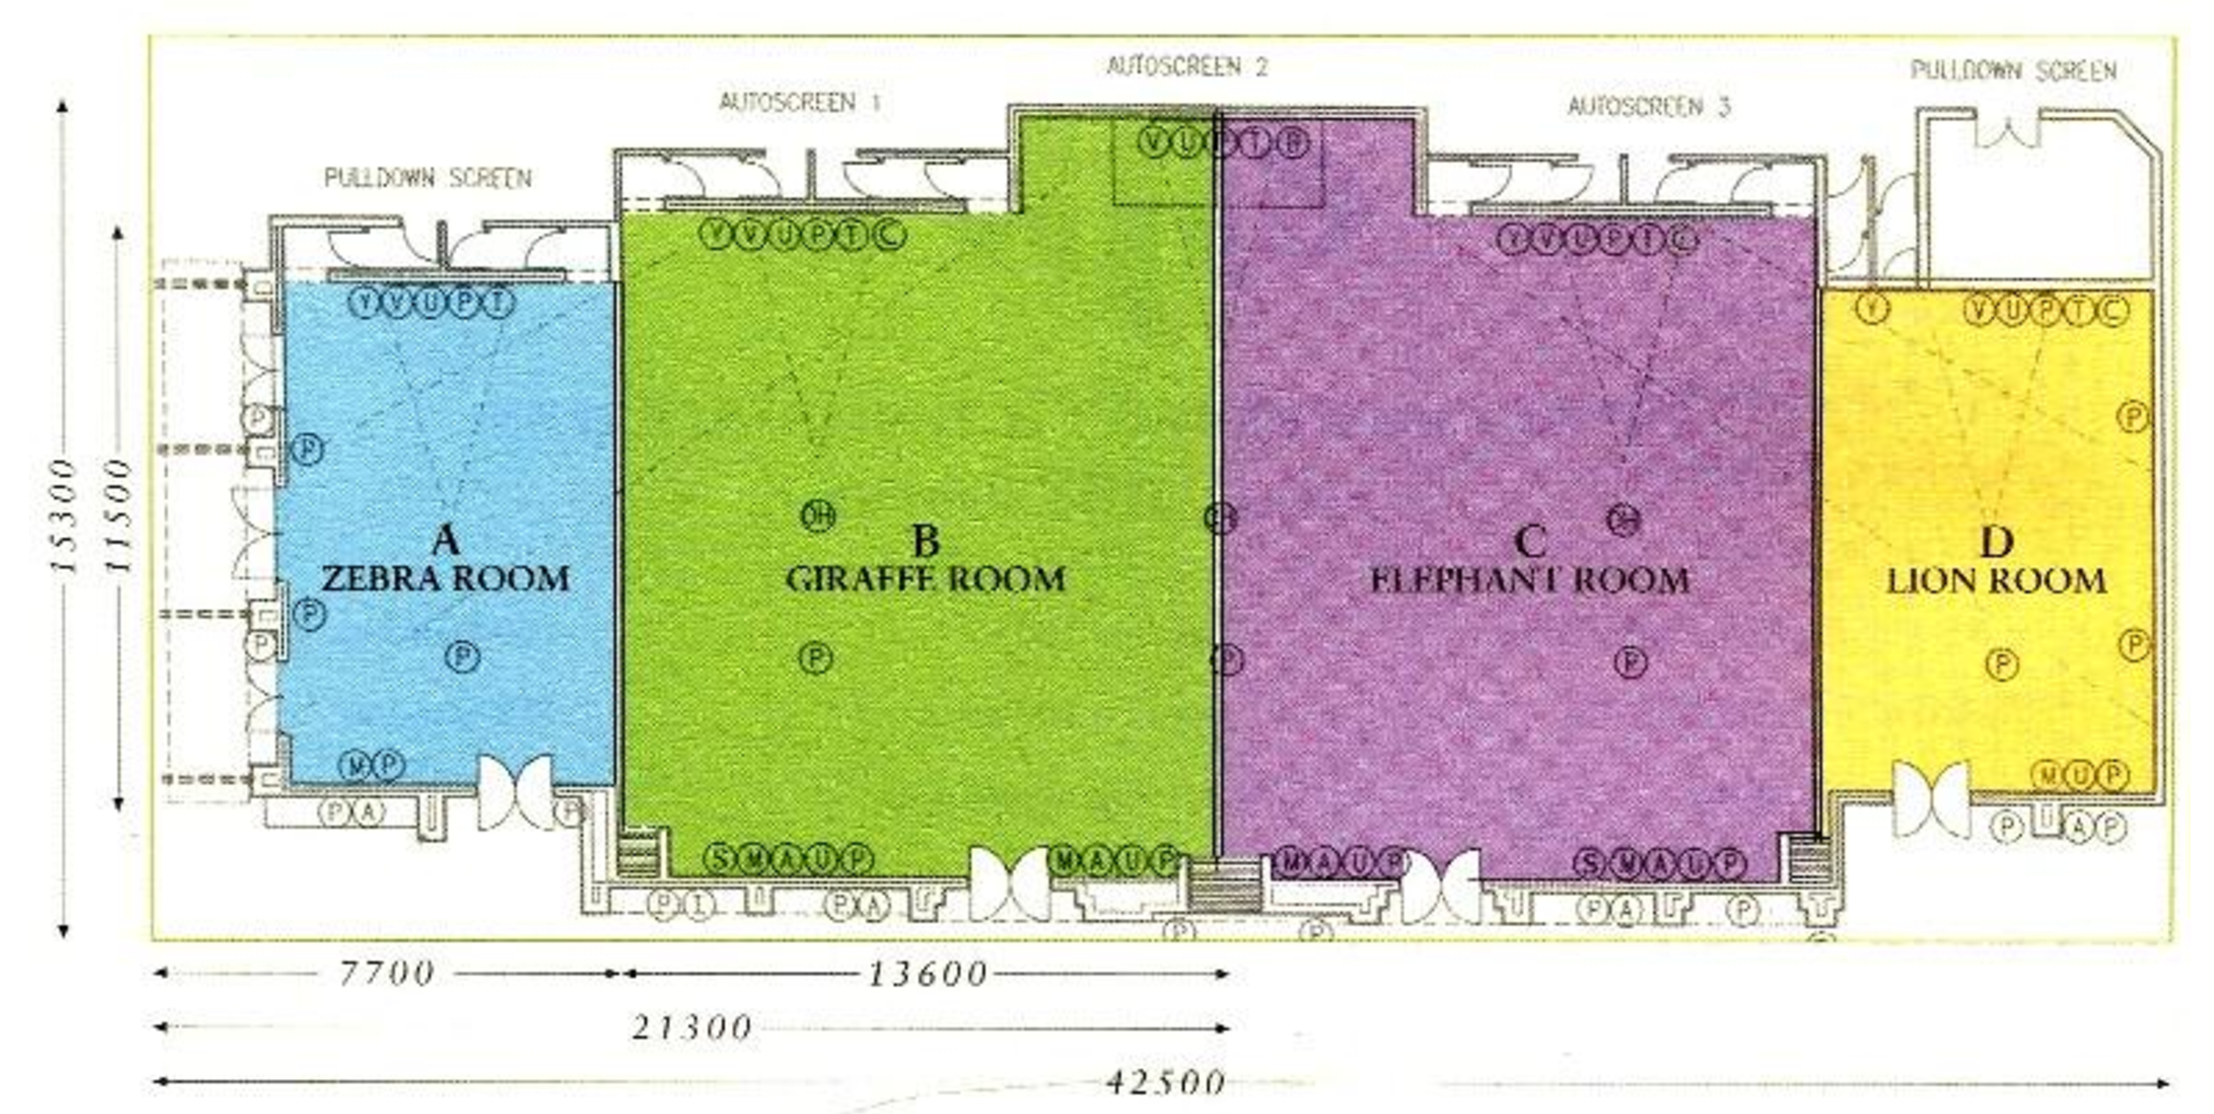
\includegraphics[width=\linewidth]{images/img-etd24-avani_victoria_fall_convention_centre_layout.png}
\end{center}


% % % % % % SPONSORS
% % % % % %------------------------------------------------------------------
% % % % % \chapter{Partner Institutions and Sponsors}
% % % % %
% % % % % \begin{center}
The ETD 2024 conference was organised by the Networked Digital Library of Theses and Dissertations (NDLTD) and, additionally hosted by The University of Zambia (UNZA) and co-hosted by The Higher Education Authority (HEA) of Zambia and Zambia Research and Education Network (ZAMREN).
\end{center}

\section{Gold, Silver and Bronze Sponsors}

\begin{center}

\includegraphics[width=0.30\textwidth]{images/logos/Partnerlogos/img-etd24-artwork-sponsors-proquest.png}

\includegraphics[width=0.30\textwidth]{images/logos/Partnerlogos/img-etd24-artwork-sponsors-ebsco.png}

\includegraphics[width=0.40\textwidth]{images/logos/Partnerlogos/img-etd24-artwork-sponsors-datacite.png}

\includegraphics[width=0.30\textwidth]{images/logos/Partnerlogos/img-etd24-artwork-sponsors-uks.png}

\includegraphics[width=0.30\textwidth]{images/logos/Partnerlogos/img-etd24-artwork-sponsors-crossref.jpg}
\includegraphics[width=0.30\textwidth]{images/logos/Partnerlogos/img-etd24-artwork-sponsors-zynle.png}
\end{center}


\section{Partner Institutions/Organisations}

\begin{center}

\includegraphics[width=0.18\textwidth]{images/logos/Partnerlogos/img-etd2024-ndltd_logo.png}

\includegraphics[width=0.10\textwidth]{images/logos/Partnerlogos/img-etd2024-unza_logo.png}

\includegraphics[width=0.18\textwidth]{images/logos/Partnerlogos/img-etd2024-hea_logo.png}

\includegraphics[width=0.25\textwidth]{images/logos/Partnerlogos/img-etd2024-zamren_logo.png}
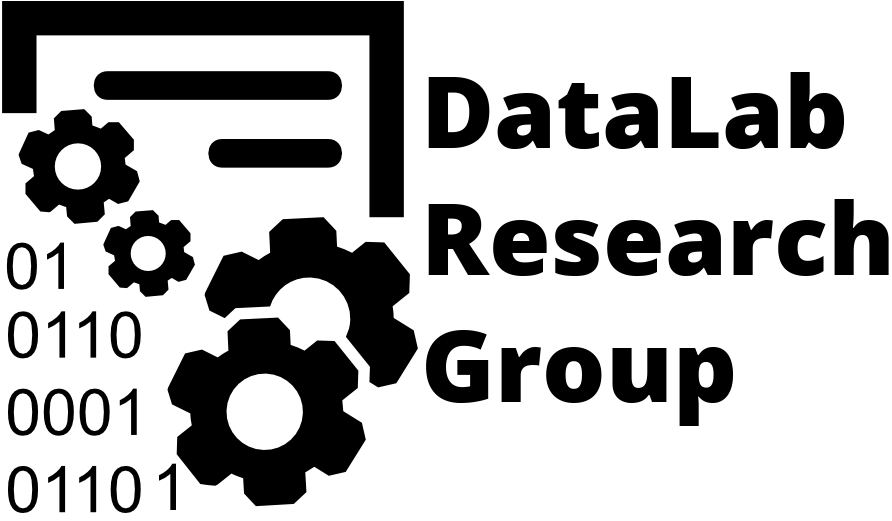
\includegraphics[width=0.18\textwidth]{images/logos/Partnerlogos/img-etd24-artwork-sponsors-datalab.png}
\end{center}


% % % % % % % % % % \vfill
% % % % %
% % % % % \section{Gold Sponsors}
% % % % %
% % % % % \begin{center}
% % % % % 
\includegraphics[width=0.20\textwidth]{images/logos/Partnerlogos/img-etd24-artwork-sponsors-proquest.png}
% % % % % \end{center}
% % % % %
% % % % % \section{Silver Sponsors}
% % % % %
% % % % % \begin{center}
% % % % % 
\includegraphics[width=0.15\textwidth]{images/logos/Partnerlogos/img-etd24-artwork-sponsors-ebsco.png}
% % % % % \end{center}
% % % % %
% % % % % \section{Bronze Sponsors}
% % % % %
% % % % % \begin{center}
% % % % % 
\includegraphics[width=0.15\textwidth]{images/logos/Partnerlogos/img-etd24-artwork-sponsors-datacite.png}
% % % % % 
\includegraphics[width=0.15\textwidth]{images/logos/Partnerlogos/img-etd24-artwork-sponsors-uks.png}
% % % % % 
\includegraphics[width=0.15\textwidth]{images/logos/Partnerlogos/img-etd24-artwork-sponsors-crossref.jpg}
% % % % % \includegraphics[width=0.15\textwidth]{images/logos/Partnerlogos/img-etd24-artwork-sponsors-zynle.png}
% % % % % \end{center}
% % % % %
% % % % % \section{Additional Sponsors}
% % % % %
% % % % % \begin{center}
% % % % % 
\includegraphics[width=0.10\textwidth]{images/logos/Partnerlogos/img-etd2024-ndltd_logo.png}
% % % % % 
\includegraphics[width=0.10\textwidth]{images/logos/Partnerlogos/img-etd2024-unza_logo.png}
% % % % % 
\includegraphics[width=0.10\textwidth]{images/logos/Partnerlogos/img-etd2024-hea_logo.png}
% % % % % 
\includegraphics[width=0.10\textwidth]{images/logos/Partnerlogos/img-etd2024-zamren_logo.png}
% % % % % 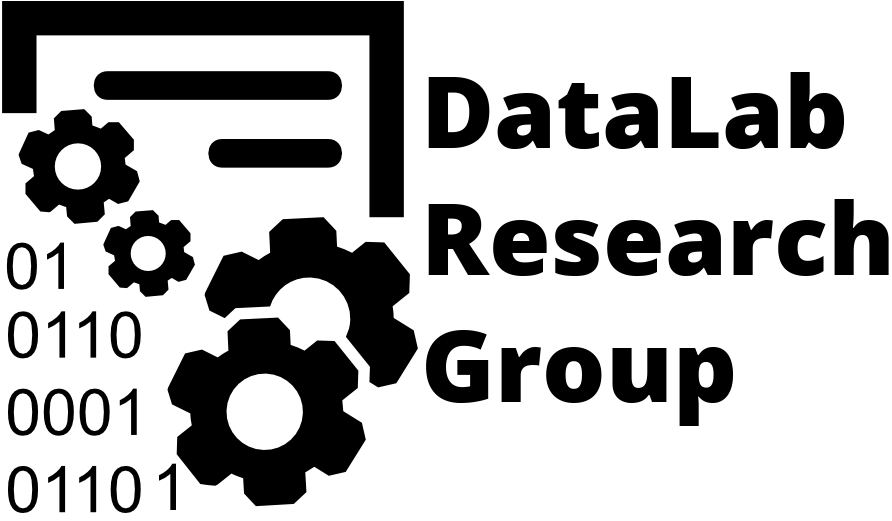
\includegraphics[width=0.10\textwidth]{images/logos/Partnerlogos/img-etd24-artwork-sponsors-datalab.png}
% % % % % \end{center}
% % % % %
% % % % % % % % % % \vfill

% % % % %
% % % % % \newpage

% BACK PAGE
%-----------------------------------------------------------------

\pagecolor{myblue}
\thispagestyle{empty}
\mbox{}

\end{document}
